\chapter{My Recollection of Professor G. Ramachandran}\label{chap6}
\vskip -0.25cm

\Authorline{N G Deshpande}

\authinfo{Professor of Physics, University of Oregon, USA.}
\vskip -0.25cm

I met Professor G. Ramachandran in early 1960s when we were both students with Professor Alladi Ramakrishnan.  Ramachandran was one of the earliest participants in the Theoretical Seminars that took place at Professor Alladi Ramakrishnan’s residence, Ekamra  Nivas in Madras. I overlapped with Ramachandran in the period 1960-61. This was one of the most exciting times in our lives. Professor Alladi Ramakkrishnan would call the Seminars almost every day, usually in the afternoon. Professor V. Devanathan was the coordinator, but topics would often depend on what discussions would arise on  the previous day. There were in general about ten to twelve participants at any given time. There were about half a dozen students like us and then there were senior faculty with Ph.D. degrees. Among the young I recall students like Balachandran, Bhamati, Radha, Thunga, Indumathi, Raman and Ramachandran. Among the seniors we had Devanathan, Venkatesan, Ranganathan, Vasudevan and Srinivasan. Professor Alladi Ramakrishnan was always present would be a very attentive and ask good questions. The topics of discussion ranged widely from new particles discovered to topics in nuclear scattering and statistical mechanics. This was a period in Physics of great new discoveries and the atmosphere was such that our interests were not compartmentalized. There was no concept of a thesis advisor so you could work on any topic with whoever was interested in that topic. Since everything was a recent discovery, there was an abundance of problems one could work on. No wonder that in this stimulating atmosphere, students went on to do path breaking work in their chosen topics. Ramachandran was interested in topics on pion scattering on nuclei and photo production. My own interest was in  elementary particles and conservation laws. 

Another noteworthy feature of those early times was the opportunity to see some of the great physicists of the time and interact with them. It is still a wonder how Professor Alladi Ramakrishnan convinced these great dignitaries to come to Madras and give lectures at his residence. I remember the visit of Professor Salam, Professor Gell-Mann, Professor Dalitz and Professor Dallaporta. Later on after the Institute of Mathematical Science was formed, seminars took place in the Institute. Many distinguished visitors have graced the new Institute.

I remember Ramachandran as a quiet and studious young man. He was a few years senior to me having obtained his M.Sc.\ In 1957 . Ramachandran’s early work was with Devanathan on photoproduction of pions on nuclei. This led to his life long interest in intermediate energy physics. He made many important contributions to this field. Among his most significant works is Delta production in inelastic nucleon nucleus collision and pion production in nucleon  nucleon  collision.  Ramachandran had a very successful career, writing more than 90 papers. After becoming Professor at Mysore University he mentored many talented students who also have had very successful  research careers.

\vspace{.7cm}

\centerline{\includegraphics[scale=1.6]{authorsphotos/N_G_Deshpande.eps}}  
\bigskip

\noindent
\textbf{Dr.\ Nilendra Deshpande} was a founder member of the Theoretical Physics Seminar Group. He later received Ph.D. in 1965 from University of Pennsylvania, USA. Since 1975 he is at the Department of Physics, University of Oregon, USA, where he is currently Professor Emeritus.
